\section{Introduction}

The Pygmy flight computer is a telemetry logging flight computer for amateur rocketry, in the Tripoli L1/L2 flight
categories. It is radio capable and based on the RP2040 microcontroller chip.

\begin{figure}[H]
    \centering
    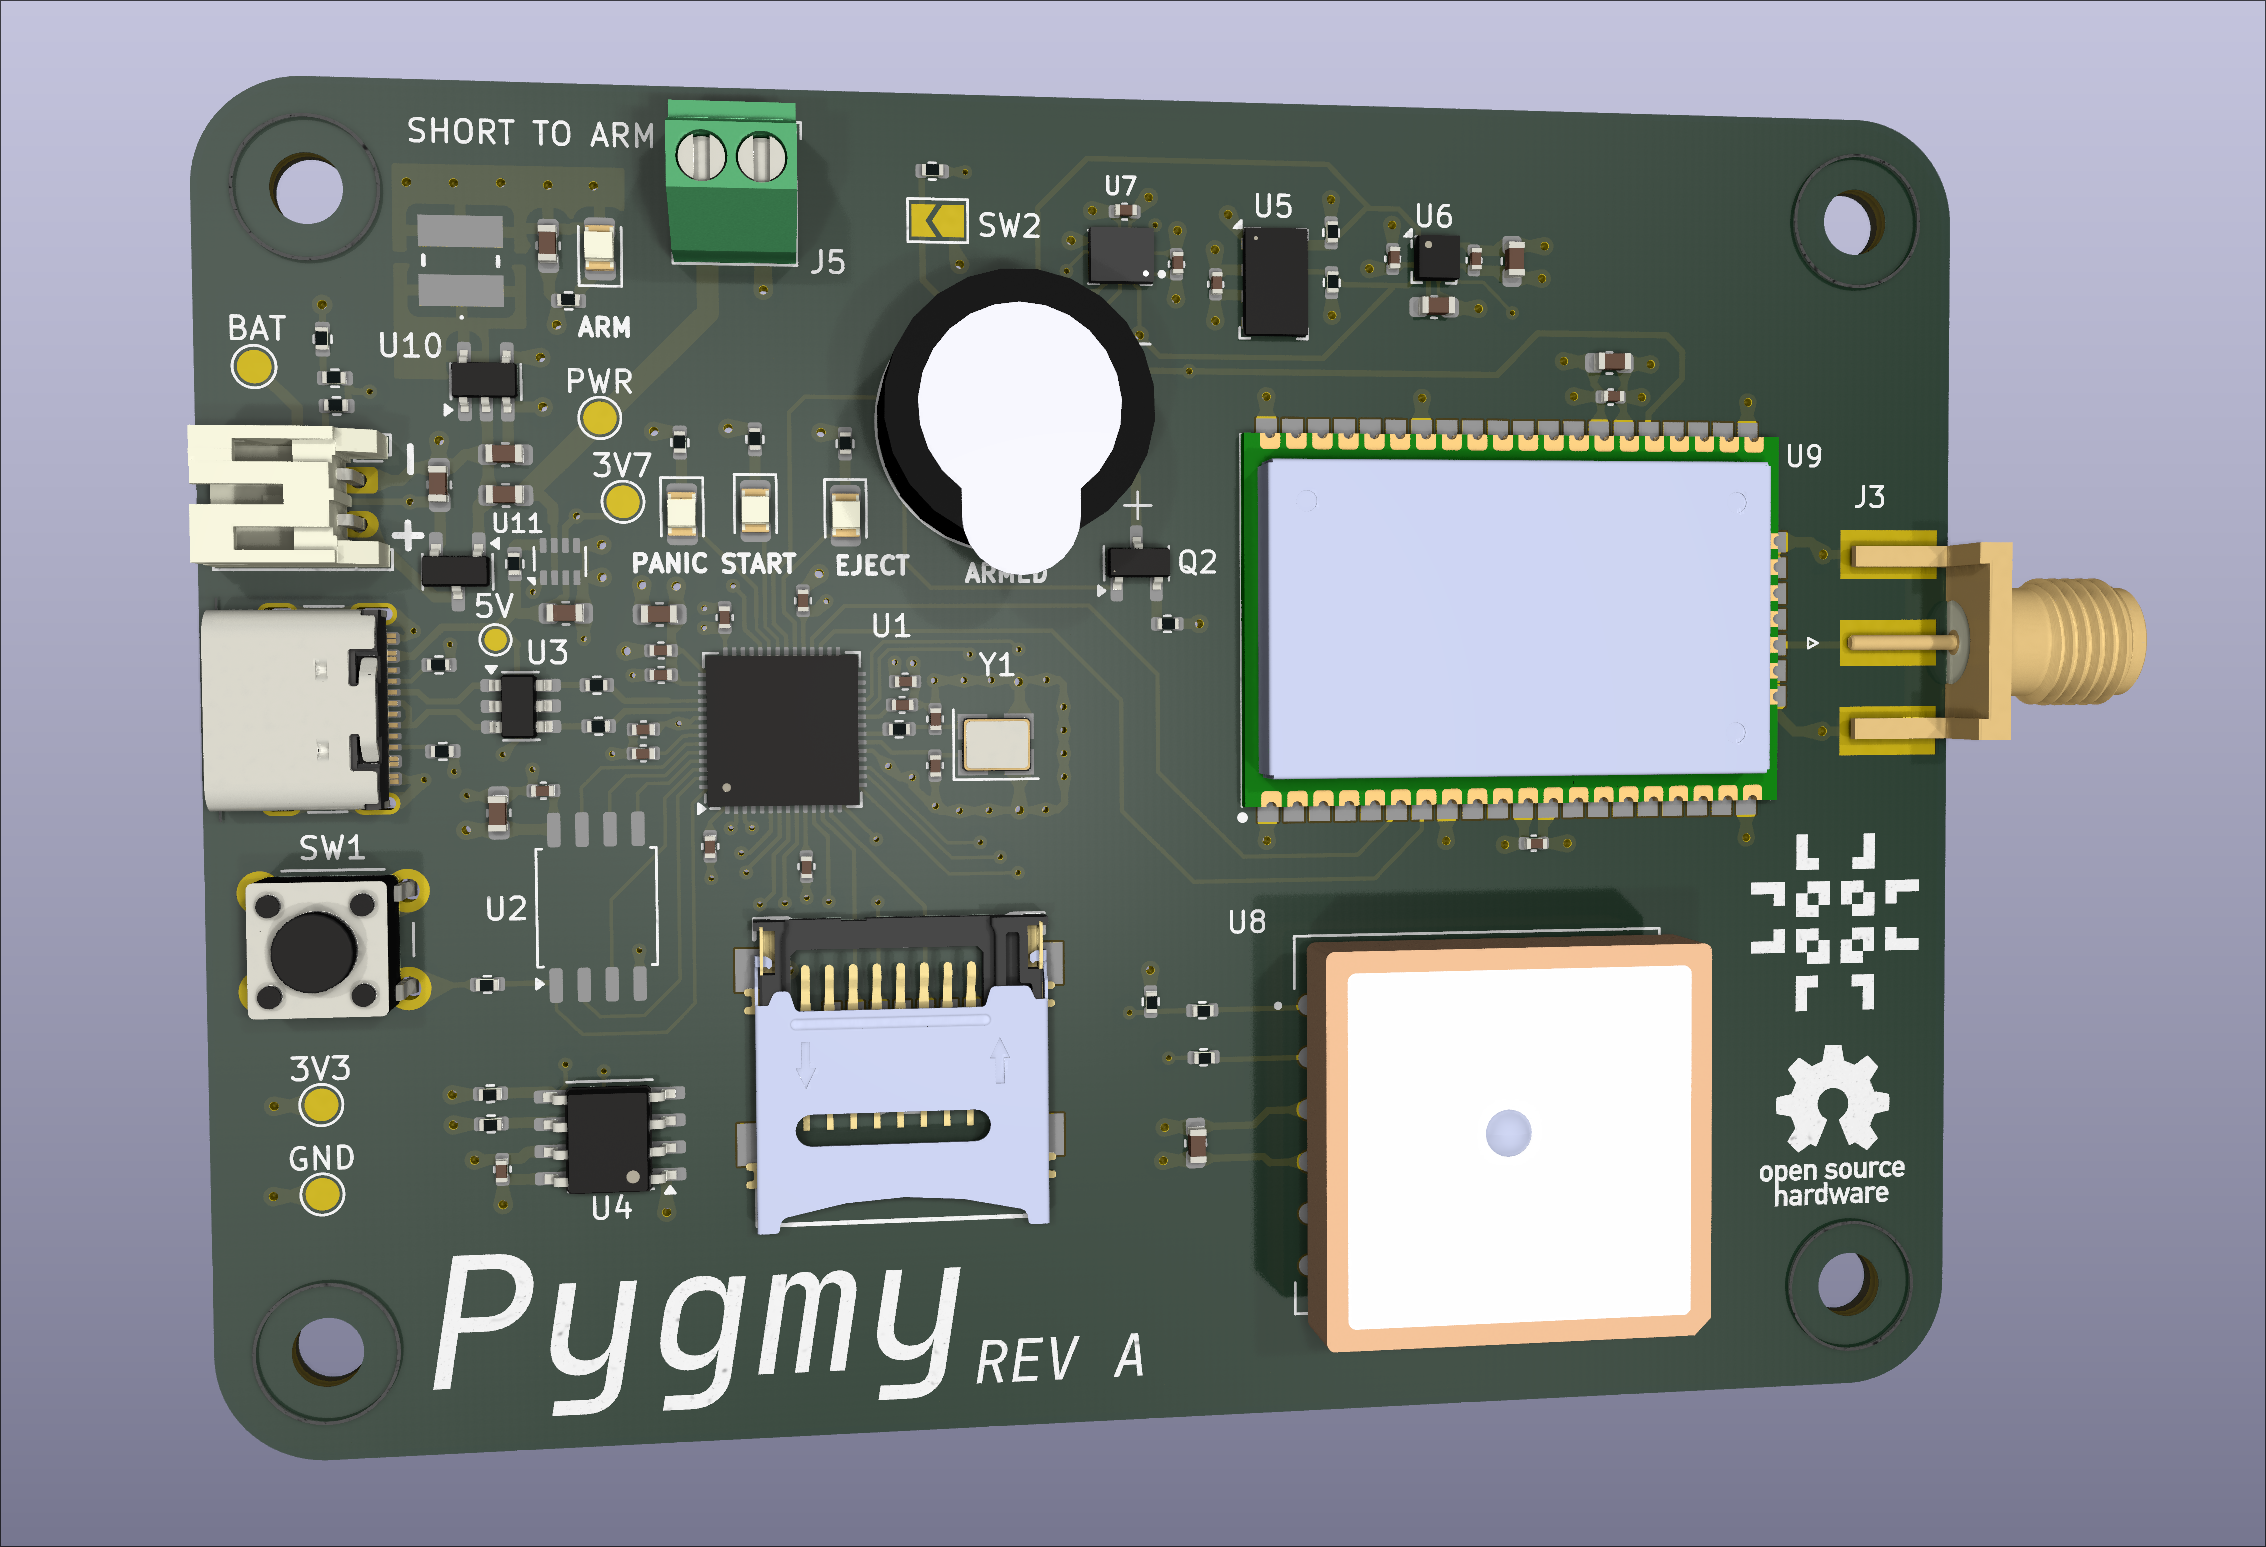
\includegraphics[width=4in]{../assets/pygmy.png}
    \caption{The Pygmy flight computer E-CAD render}
\end{figure}

The Pygmy flight computer has been designed to be a feature-packed telemetry flight computer capable of handling
flights where space is tight and data collection is critical. It has the following key features:

\begin{itemize}
    \item RP2040 microcontroller with 2MB flash
    \item USB-C port for bench power, programming and a debug console
    \item JST battery connector for 3.7V 18650 or LiPo battery power
    \item Arming terminal
    \item Micro SD card with only 1 microsecond of discontinuity under 50g of force
    \item RN2903 915MHz LoRa radio transceiver with SMA connector
    \item L86G GPS receiver with passive patch antenna
    \item MS5607 barometric pressure sensor with 2.4Pa resolution and range of 120kPa to 1kPa
    \item LIS2MDL magnetometer
    \item LSM6DSO32 6-axis IMU with up to $\pm$32g full scale
    \item 32Kbit EEPROM for calibration settings
    \item Piezoelectric buzzer for auditory status indication
    \item Battery charge monitor via RP2040 ADC
\end{itemize}
